% Generated by ArticleSignalDiagrams. Opaque vector fills only.
\documentclass[10pt,tikz,border=5pt]{standalone}
\usepackage{lmodern}
\usetikzlibrary{fit}
\begin{document}
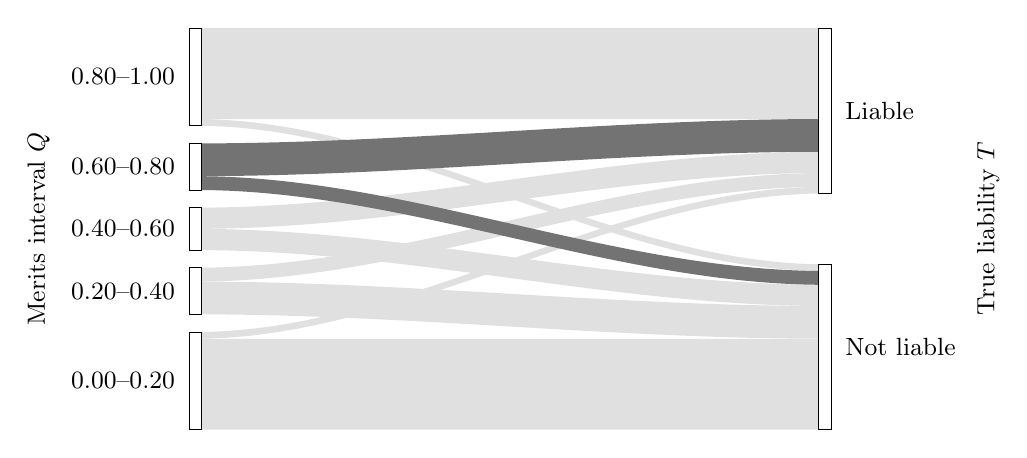
\begin{tikzpicture}[x=1cm,y=1cm,font=\small]\path[fill=black!12,draw=none] (3.3,-5.1) .. controls (6,-5.1) and (8.6,-5.1) .. (11.3,-5.1) -- (11.3,-3.945388) .. controls (8.6,-3.945388) and (6,-3.945388) .. (3.3,-3.945388) -- cycle;
\path[fill=black!12,draw=none] (3.3,-3.945388) .. controls (6,-3.945388) and (8.6,-2.1) .. (11.3,-2.1) -- (11.3,-2.014909) .. controls (8.6,-2.014909) and (6,-3.860298) .. (3.3,-3.860298) -- cycle;
\path[fill=black!12,draw=none] (3.3,-3.635298) .. controls (6,-3.635298) and (8.6,-3.945388) .. (11.3,-3.945388) -- (11.3,-3.529653) .. controls (8.6,-3.529653) and (6,-3.219562) .. (3.3,-3.219562) -- cycle;
\path[fill=black!12,draw=none] (3.3,-3.219562) .. controls (6,-3.219562) and (8.6,-2.014909) .. (11.3,-2.014909) -- (11.3,-1.839543) .. controls (8.6,-1.839543) and (6,-3.044196) .. (3.3,-3.044196) -- cycle;
\path[fill=black!12,draw=none] (3.3,-2.819196) .. controls (6,-2.819196) and (8.6,-3.529653) .. (11.3,-3.529653) -- (11.3,-3.260457) .. controls (8.6,-3.260457) and (6,-2.55) .. (3.3,-2.55) -- cycle;
\path[fill=black!12,draw=none] (3.3,-2.55) .. controls (6,-2.55) and (8.6,-1.839543) .. (11.3,-1.839543) -- (11.3,-1.570347) .. controls (8.6,-1.570347) and (6,-2.280804) .. (3.3,-2.280804) -- cycle;
\path[fill=black!12,draw=none] (3.3,-1.239702) .. controls (6,-1.239702) and (8.6,-3.085091) .. (11.3,-3.085091) -- (11.3,-3) .. controls (8.6,-3) and (6,-1.154612) .. (3.3,-1.154612) -- cycle;
\path[fill=black!12,draw=none] (3.3,-1.154612) .. controls (6,-1.154612) and (8.6,-1.154612) .. (11.3,-1.154612) -- (11.3,-0) .. controls (8.6,-0) and (6,-0) .. (3.3,-0) -- cycle;
\path[fill=black!55,draw=none] (3.3,-2.055804) .. controls (6,-2.055804) and (8.6,-3.260457) .. (11.3,-3.260457) -- (11.3,-3.085091) .. controls (8.6,-3.085091) and (6,-1.880438) .. (3.3,-1.880438) -- cycle;
\path[fill=black!55,draw=none] (3.3,-1.880438) .. controls (6,-1.880438) and (8.6,-1.570347) .. (11.3,-1.570347) -- (11.3,-1.154612) .. controls (8.6,-1.154612) and (6,-1.464702) .. (3.3,-1.464702) -- cycle;
\coordinate (axis-midline-0) at (0,-2.55);
\path[fill=white,draw=black,line width=0.3pt] (3.22,-5.1) rectangle (3.38,-3.860298);
\node[anchor=east,fill=white,inner sep=2pt] (bucket-0-0-0) at (3.12,-4.480149) {0.00--0.20};
\path[fill=white,draw=black,line width=0.3pt] (3.22,-3.635298) rectangle (3.38,-3.044196);
\node[anchor=east,fill=white,inner sep=2pt] (bucket-0-0-1) at (3.12,-3.339747) {0.20--0.40};
\path[fill=white,draw=black,line width=0.3pt] (3.22,-2.819196) rectangle (3.38,-2.280804);
\node[anchor=east,fill=white,inner sep=2pt] (bucket-0-0-2) at (3.12,-2.55) {0.40--0.60};
\path[fill=white,draw=black,line width=0.3pt] (3.22,-2.055804) rectangle (3.38,-1.464702);
\node[anchor=east,fill=white,inner sep=2pt] (bucket-0-0-3) at (3.12,-1.760253) {0.60--0.80};
\path[fill=white,draw=black,line width=0.3pt] (3.22,-1.239702) rectangle (3.38,-0);
\node[anchor=east,fill=white,inner sep=2pt] (bucket-0-0-4) at (3.12,-0.619851) {0.80--1.00};
\node[fit=(bucket-0-0-0) (bucket-0-0-1) (bucket-0-0-2) (bucket-0-0-3) (bucket-0-0-4),inner sep=0pt] (source-labels-0) {};
\coordinate (axis-title-0-0) at (source-labels-0.west |- axis-midline-0);
\node[rotate=90,anchor=south,inner sep=0pt] at ([xshift=-0.18cm]axis-title-0-0) {Merits interval $Q$};
\path[fill=white,draw=black,line width=0.3pt] (11.22,-5.1) rectangle (11.38,-3);
\node[anchor=west,fill=white,inner sep=2pt] (bucket-0-1-0) at (11.48,-4.05) {Not liable};
\path[fill=white,draw=black,line width=0.3pt] (11.22,-2.1) rectangle (11.38,-0);
\node[anchor=west,fill=white,inner sep=2pt] (bucket-0-1-1) at (11.48,-1.05) {Liable};
\node[fit=(bucket-0-1-0) (bucket-0-1-1),inner sep=0pt] (destination-labels-0) {};
\coordinate (axis-title-0-1) at (destination-labels-0.east |- axis-midline-0);
\node[rotate=90,anchor=north,inner sep=0pt] at ([xshift=0.18cm]axis-title-0-1) {True liability $T$};
\end{tikzpicture}
\end{document}

